% Generated by scripts/make_crossed_figure.py; do not edit.
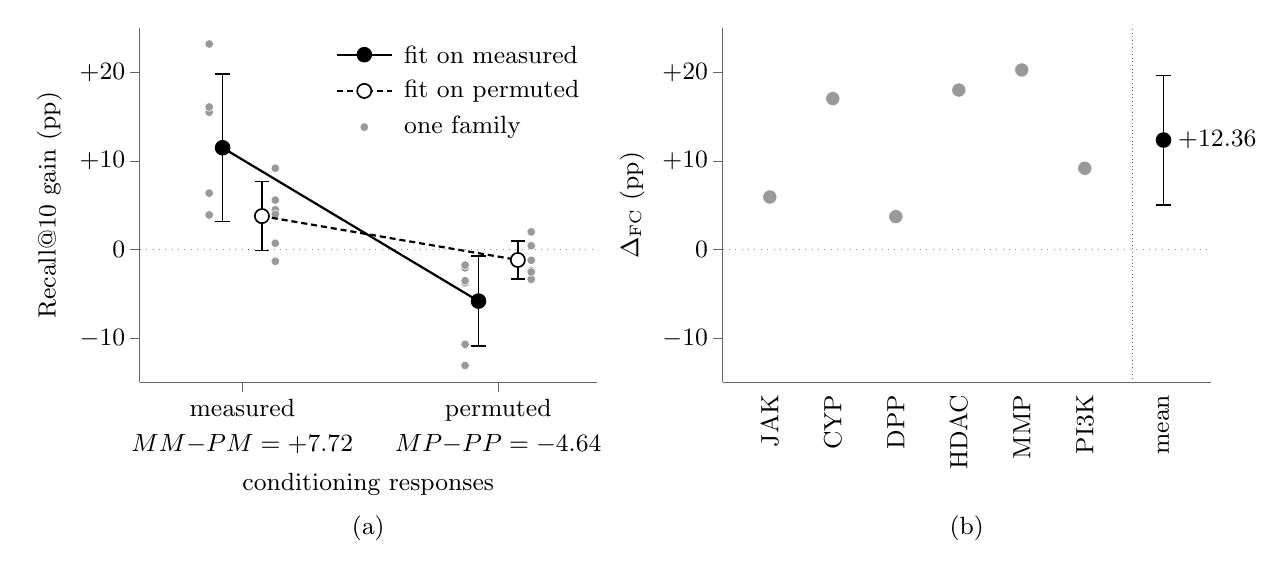
\begin{tikzpicture}[x=1mm,y=1mm,
    ax/.style={black!60,line width=0.3pt},
    zero/.style={black!45,line width=0.3pt,dotted},
    bar/.style={black,line width=0.5pt},
    fitM/.style={black,line width=0.8pt},
    fitP/.style={black,line width=0.8pt,dash pattern=on 2.2pt off 1.4pt},
    meanM/.style={fill=black,draw=black,line width=0.5pt},
    meanP/.style={fill=white,draw=black,line width=0.6pt},
    fam/.style={fill=black!40,draw=white,line width=0.2pt}]
  %% panel (a): Recall@10 gain by fitting x conditioning
  \draw[ax] (0.0,0.00) -- (0.0,45.00);
  \draw[ax] (0.0,5.62) -- (-1.2,5.62);
  \node[anchor=east,font=\small,inner sep=0.6mm] at (-1.2,5.62) {$-10$};
  \draw[ax] (0.0,16.88) -- (-1.2,16.88);
  \node[anchor=east,font=\small,inner sep=0.6mm] at (-1.2,16.88) {$0$};
  \draw[ax] (0.0,28.12) -- (-1.2,28.12);
  \node[anchor=east,font=\small,inner sep=0.6mm] at (-1.2,28.12) {$+10$};
  \draw[ax] (0.0,39.38) -- (-1.2,39.38);
  \node[anchor=east,font=\small,inner sep=0.6mm] at (-1.2,39.38) {$+20$};
  \node[rotate=90,font=\small] at (-11.5,22.50) {Recall@10 gain (pp)};
  \draw[zero] (0,16.88) -- (58.0,16.88);
  \draw[ax] (0,0.00) -- (58.0,0.00);
  \draw[ax] (13.0,0.00) -- (13.0,-1.20);
  \node[anchor=north,font=\small,inner sep=0pt] at (13.0,-2.00) {measured};
  \node[anchor=north,font=\small,inner sep=0pt] at (13.0,-6.50) {$MM{-}PM=+7.72$};
  \draw[ax] (45.5,0.00) -- (45.5,-1.20);
  \node[anchor=north,font=\small,inner sep=0pt] at (45.5,-2.00) {permuted};
  \node[anchor=north,font=\small,inner sep=0pt] at (45.5,-6.50) {$MP{-}PP=-4.64$};
  \node[anchor=north,font=\small,inner sep=0pt] at (29.0,-11.50) {conditioning responses};
  \fill[fam] (8.80,24.04) circle (0.55mm);
  \fill[fam] (8.80,34.32) circle (0.55mm);
  \fill[fam] (8.80,21.23) circle (0.55mm);
  \fill[fam] (8.80,42.98) circle (0.55mm);
  \fill[fam] (8.80,34.98) circle (0.55mm);
  \fill[fam] (8.80,21.27) circle (0.55mm);
  \fill[fam] (41.30,14.55) circle (0.55mm);
  \fill[fam] (41.30,2.15) circle (0.55mm);
  \fill[fam] (41.30,14.90) circle (0.55mm);
  \fill[fam] (41.30,12.66) circle (0.55mm);
  \fill[fam] (41.30,4.83) circle (0.55mm);
  \fill[fam] (41.30,12.92) circle (0.55mm);
  \fill[fam] (17.20,21.93) circle (0.55mm);
  \fill[fam] (17.20,27.20) circle (0.55mm);
  \fill[fam] (17.20,17.67) circle (0.55mm);
  \fill[fam] (17.20,23.16) circle (0.55mm);
  \fill[fam] (17.20,21.36) circle (0.55mm);
  \fill[fam] (17.20,15.38) circle (0.55mm);
  \fill[fam] (49.70,19.12) circle (0.55mm);
  \fill[fam] (49.70,14.19) circle (0.55mm);
  \fill[fam] (49.70,15.51) circle (0.55mm);
  \fill[fam] (49.70,13.10) circle (0.55mm);
  \fill[fam] (49.70,14.02) circle (0.55mm);
  \fill[fam] (49.70,17.36) circle (0.55mm);
  \draw[fitM] (10.50,29.80) -- (43.00,10.33);
  \draw[fitP] (15.50,21.12) -- (48.00,15.55);
  \draw[bar] (10.50,20.41) -- (10.50,39.19);
  \draw[bar] (9.60,20.41) -- (11.40,20.41);
  \draw[bar] (9.60,39.19) -- (11.40,39.19);
  \filldraw[meanM] (10.50,29.80) circle (0.9mm);
  \draw[bar] (43.00,4.63) -- (43.00,16.04);
  \draw[bar] (42.10,4.63) -- (43.90,4.63);
  \draw[bar] (42.10,16.04) -- (43.90,16.04);
  \filldraw[meanM] (43.00,10.33) circle (0.9mm);
  \draw[bar] (15.50,16.75) -- (15.50,25.49);
  \draw[bar] (14.60,16.75) -- (16.40,16.75);
  \draw[bar] (14.60,25.49) -- (16.40,25.49);
  \filldraw[meanP] (15.50,21.12) circle (0.9mm);
  \draw[bar] (48.00,13.15) -- (48.00,17.95);
  \draw[bar] (47.10,13.15) -- (48.90,13.15);
  \draw[bar] (47.10,17.95) -- (48.90,17.95);
  \filldraw[meanP] (48.00,15.55) circle (0.9mm);
  \draw[fitM] (25.0,41.62) -- (32.0,41.62);
  \filldraw[meanM] (28.5,41.62) circle (0.9mm);
  \node[anchor=west,font=\small,inner sep=0pt] at (33.5,41.62) {fit on measured};
  \draw[fitP] (25.0,37.02) -- (32.0,37.02);
  \filldraw[meanP] (28.5,37.02) circle (0.9mm);
  \node[anchor=west,font=\small,inner sep=0pt] at (33.5,37.02) {fit on permuted};
  \fill[fam] (28.5,32.42) circle (0.55mm);
  \node[anchor=west,font=\small,inner sep=0pt] at (33.5,32.42) {one family};
  \node[font=\small] at (29.0,-18.50) {(a)};
  %% panel (b): per-family interaction
  \draw[ax] (74.0,0.00) -- (74.0,45.00);
  \draw[ax] (74.0,5.62) -- (72.8,5.62);
  \node[anchor=east,font=\small,inner sep=0.6mm] at (72.8,5.62) {$-10$};
  \draw[ax] (74.0,16.88) -- (72.8,16.88);
  \node[anchor=east,font=\small,inner sep=0.6mm] at (72.8,16.88) {$0$};
  \draw[ax] (74.0,28.12) -- (72.8,28.12);
  \node[anchor=east,font=\small,inner sep=0.6mm] at (72.8,28.12) {$+10$};
  \draw[ax] (74.0,39.38) -- (72.8,39.38);
  \node[anchor=east,font=\small,inner sep=0.6mm] at (72.8,39.38) {$+20$};
  \node[rotate=90,font=\small] at (62.5,22.50) {$\Delta_{\mathrm{FC}}$ (pp)};
  \draw[zero] (74.0,16.88) -- (136.0,16.88);
  \draw[ax] (74.0,0.00) -- (136.0,0.00);
  \fill[fam] (80.0,23.55) circle (0.9mm);
  \node[rotate=90,anchor=east,font=\small,inner sep=0pt] at (80.0,-1.50) {JAK};
  \fill[fam] (88.0,36.04) circle (0.9mm);
  \node[rotate=90,anchor=east,font=\small,inner sep=0pt] at (88.0,-1.50) {CYP};
  \fill[fam] (96.0,21.05) circle (0.9mm);
  \node[rotate=90,anchor=east,font=\small,inner sep=0pt] at (96.0,-1.50) {DPP};
  \fill[fam] (104.0,37.13) circle (0.9mm);
  \node[rotate=90,anchor=east,font=\small,inner sep=0pt] at (104.0,-1.50) {HDAC};
  \fill[fam] (112.0,39.68) circle (0.9mm);
  \node[rotate=90,anchor=east,font=\small,inner sep=0pt] at (112.0,-1.50) {MMP};
  \fill[fam] (120.0,27.20) circle (0.9mm);
  \node[rotate=90,anchor=east,font=\small,inner sep=0pt] at (120.0,-1.50) {PI3K};
  \draw[ax,densely dotted] (126.0,0.00) -- (126.0,45.00);
  \draw[bar] (130.00,22.55) -- (130.00,39.00);
  \draw[bar] (129.10,22.55) -- (130.90,22.55);
  \draw[bar] (129.10,39.00) -- (130.90,39.00);
  \filldraw[meanM] (130.0,30.78) circle (0.9mm);
  \node[anchor=west,font=\small,inner sep=0pt] at (131.8,30.78) {$+12.36$};
  \node[rotate=90,anchor=east,font=\small,inner sep=0pt] at (130.0,-1.50) {mean};
  \node[font=\small] at (105.0,-18.50) {(b)};
\end{tikzpicture}
